\documentclass{article}\usepackage[]{graphicx}\usepackage[]{color}
%% maxwidth is the original width if it is less than linewidth
%% otherwise use linewidth (to make sure the graphics do not exceed the margin)
\makeatletter
\def\maxwidth{ %
  \ifdim\Gin@nat@width>\linewidth
    \linewidth
  \else
    \Gin@nat@width
  \fi
}
\makeatother

\definecolor{fgcolor}{rgb}{0.345, 0.345, 0.345}
\newcommand{\hlnum}[1]{\textcolor[rgb]{0.686,0.059,0.569}{#1}}%
\newcommand{\hlstr}[1]{\textcolor[rgb]{0.192,0.494,0.8}{#1}}%
\newcommand{\hlcom}[1]{\textcolor[rgb]{0.678,0.584,0.686}{\textit{#1}}}%
\newcommand{\hlopt}[1]{\textcolor[rgb]{0,0,0}{#1}}%
\newcommand{\hlstd}[1]{\textcolor[rgb]{0.345,0.345,0.345}{#1}}%
\newcommand{\hlkwa}[1]{\textcolor[rgb]{0.161,0.373,0.58}{\textbf{#1}}}%
\newcommand{\hlkwb}[1]{\textcolor[rgb]{0.69,0.353,0.396}{#1}}%
\newcommand{\hlkwc}[1]{\textcolor[rgb]{0.333,0.667,0.333}{#1}}%
\newcommand{\hlkwd}[1]{\textcolor[rgb]{0.737,0.353,0.396}{\textbf{#1}}}%

\usepackage{framed}
\makeatletter
\newenvironment{kframe}{%
 \def\at@end@of@kframe{}%
 \ifinner\ifhmode%
  \def\at@end@of@kframe{\end{minipage}}%
  \begin{minipage}{\columnwidth}%
 \fi\fi%
 \def\FrameCommand##1{\hskip\@totalleftmargin \hskip-\fboxsep
 \colorbox{shadecolor}{##1}\hskip-\fboxsep
     % There is no \\@totalrightmargin, so:
     \hskip-\linewidth \hskip-\@totalleftmargin \hskip\columnwidth}%
 \MakeFramed {\advance\hsize-\width
   \@totalleftmargin\z@ \linewidth\hsize
   \@setminipage}}%
 {\par\unskip\endMakeFramed%
 \at@end@of@kframe}
\makeatother

\definecolor{shadecolor}{rgb}{.97, .97, .97}
\definecolor{messagecolor}{rgb}{0, 0, 0}
\definecolor{warningcolor}{rgb}{1, 0, 1}
\definecolor{errorcolor}{rgb}{1, 0, 0}
\newenvironment{knitrout}{}{} % an empty environment to be redefined in TeX

\usepackage{alltt}
\usepackage[sc]{mathpazo}
\usepackage[T1]{fontenc}
\usepackage{geometry}
\geometry{verbose,tmargin=2.5cm,bmargin=2.5cm,lmargin=2.5cm,rmargin=2.5cm}
\setcounter{secnumdepth}{2}
\setcounter{tocdepth}{2}
\usepackage{url}
\usepackage[unicode=true,pdfusetitle,
 bookmarks=true,bookmarksnumbered=true,bookmarksopen=true,bookmarksopenlevel=2,
 breaklinks=false,pdfborder={0 0 1},backref=false,colorlinks=false]
 {hyperref}
\hypersetup{
 pdfstartview={XYZ null null 1}}
\usepackage{breakurl}
\IfFileExists{upquote.sty}{\usepackage{upquote}}{}
\begin{document}


\section*{Problem Four}

I did this problem with two different dimensions, namely, n = 100, and n = 200, and I feel there are interesting things happening. It seems the min and max(as indicated in the problem) follows a normal distribution with mean as a function of p, and it is illustrated by the hand written sheets attached.
\begin{knitrout}
\definecolor{shadecolor}{rgb}{0.969, 0.969, 0.969}\color{fgcolor}\begin{kframe}
\begin{alltt}
\hlkwd{library}\hlstd{(compiler)}
\hlstd{X} \hlkwb{<-} \hlkwd{matrix}\hlstd{(}\hlkwd{rnorm}\hlstd{(}\hlnum{1e+05}\hlstd{),} \hlkwc{nrow} \hlstd{=} \hlnum{1000}\hlstd{)}
\hlstd{rowsqure} \hlkwb{<-} \hlkwa{function}\hlstd{(}\hlkwc{x}\hlstd{,} \hlkwc{y}\hlstd{) \{}
    \hlstd{rs} \hlkwb{<-} \hlkwd{matrix}\hlstd{(}\hlnum{NA}\hlstd{, nrow} \hlkwb{<-} \hlkwd{nrow}\hlstd{(y))}
    \hlkwa{for} \hlstd{(i} \hlkwa{in} \hlnum{1}\hlopt{:}\hlkwd{nrow}\hlstd{(y)) \{}
        \hlstd{rs[i]} \hlkwb{<-} \hlkwd{sum}\hlstd{((x} \hlopt{-} \hlstd{y[i, ])}\hlopt{^}\hlnum{2}\hlstd{)}
    \hlstd{\}}
    \hlkwd{return}\hlstd{(rs)}
\hlstd{\}}
\hlstd{Simulate} \hlkwb{<-} \hlkwa{function}\hlstd{(}\hlkwc{n}\hlstd{,} \hlkwc{X}\hlstd{) \{}
    \hlstd{min} \hlkwb{<-} \hlkwd{matrix}\hlstd{(}\hlnum{NA}\hlstd{,} \hlkwc{nrow} \hlstd{= n)}
    \hlstd{max} \hlkwb{<-} \hlkwd{matrix}\hlstd{(}\hlnum{NA}\hlstd{,} \hlkwc{nrow} \hlstd{= n)}
    \hlkwa{for} \hlstd{(k} \hlkwa{in} \hlnum{1}\hlopt{:}\hlstd{n) \{}
        \hlstd{i} \hlkwb{<-} \hlkwd{sample}\hlstd{(}\hlkwd{c}\hlstd{(}\hlnum{1}\hlopt{:}\hlnum{1000}\hlstd{),} \hlnum{1}\hlstd{)}
        \hlstd{min[k]} \hlkwb{<-} \hlkwd{min}\hlstd{(}\hlkwd{rowsqure}\hlstd{(X[i, ], X[}\hlopt{-}\hlstd{i, ]))}\hlopt{/}\hlnum{10}
        \hlstd{max[k]} \hlkwb{<-} \hlkwd{max}\hlstd{(}\hlkwd{rowsqure}\hlstd{(X[i, ], X[}\hlopt{-}\hlstd{i, ]))}\hlopt{/}\hlnum{10}
    \hlstd{\}}
    \hlkwd{return}\hlstd{(}\hlkwd{data.frame}\hlstd{(}\hlkwc{min} \hlstd{= min,} \hlkwc{max} \hlstd{= max))}
\hlstd{\}}
\hlstd{Simulation} \hlkwb{<-} \hlkwd{Simulate}\hlstd{(}\hlnum{1000}\hlstd{, X)}
\hlkwd{par}\hlstd{(}\hlkwc{mfcol} \hlstd{=} \hlkwd{c}\hlstd{(}\hlnum{1}\hlstd{,} \hlnum{2}\hlstd{))}
\hlkwd{hist}\hlstd{(Simulation}\hlopt{$}\hlstd{min,} \hlkwc{main} \hlstd{=} \hlstr{"min dimension 100"}\hlstd{)}
\hlkwd{hist}\hlstd{(Simulation}\hlopt{$}\hlstd{max,} \hlkwc{main} \hlstd{=} \hlstr{"max dimension 100"}\hlstd{)}
\end{alltt}
\end{kframe}
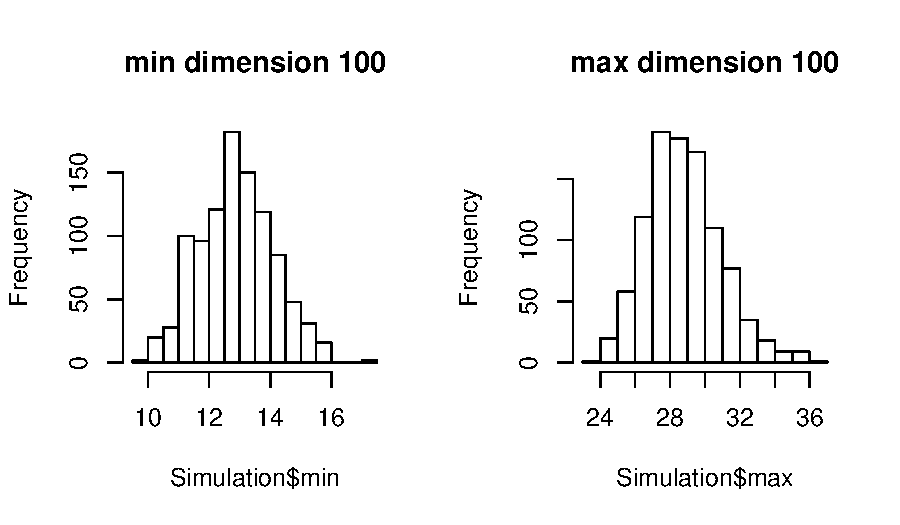
\includegraphics[width=\maxwidth]{figure/minimal-Problem_41} 
\begin{kframe}\begin{alltt}
\hlcom{# Now I increase the dimension of X to 200}
\hlstd{X_new} \hlkwb{<-} \hlkwd{matrix}\hlstd{(}\hlkwd{rnorm}\hlstd{(}\hlnum{2e+05}\hlstd{),} \hlkwc{nrow} \hlstd{=} \hlnum{1000}\hlstd{)}
\hlstd{Simulation_1} \hlkwb{<-} \hlkwd{Simulate}\hlstd{(}\hlnum{1000}\hlstd{, X_new)}
\hlkwd{hist}\hlstd{(Simulation_1}\hlopt{$}\hlstd{min,} \hlkwc{main} \hlstd{=} \hlstr{"min dimension 200"}\hlstd{)}
\hlkwd{hist}\hlstd{(Simulation_1}\hlopt{$}\hlstd{max,} \hlkwc{main} \hlstd{=} \hlstr{"max dimension 200"}\hlstd{)}
\end{alltt}
\end{kframe}
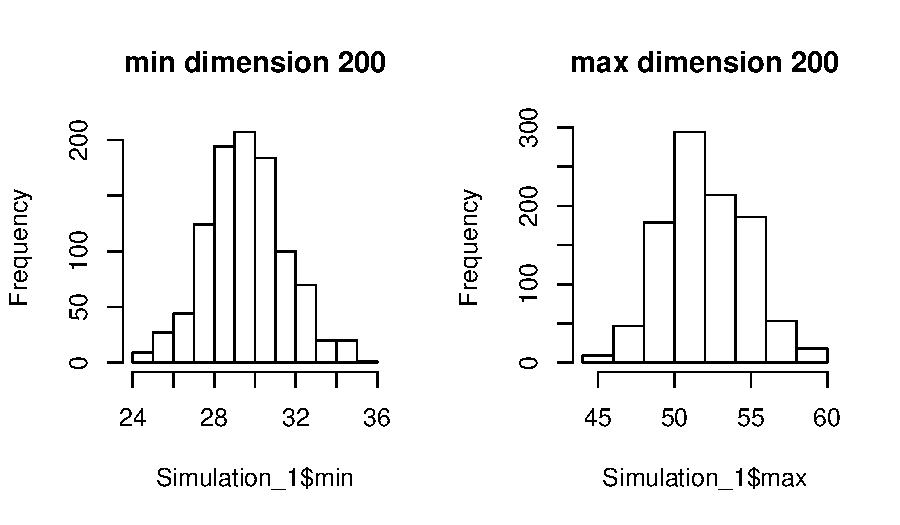
\includegraphics[width=\maxwidth]{figure/minimal-Problem_42} 
\begin{kframe}\begin{alltt}

\end{alltt}
\end{kframe}
\end{knitrout}

\end{document}
